\section{Evaluation}
\label{sec:evaluation}

\begin{figure*}[!tb]
  \center
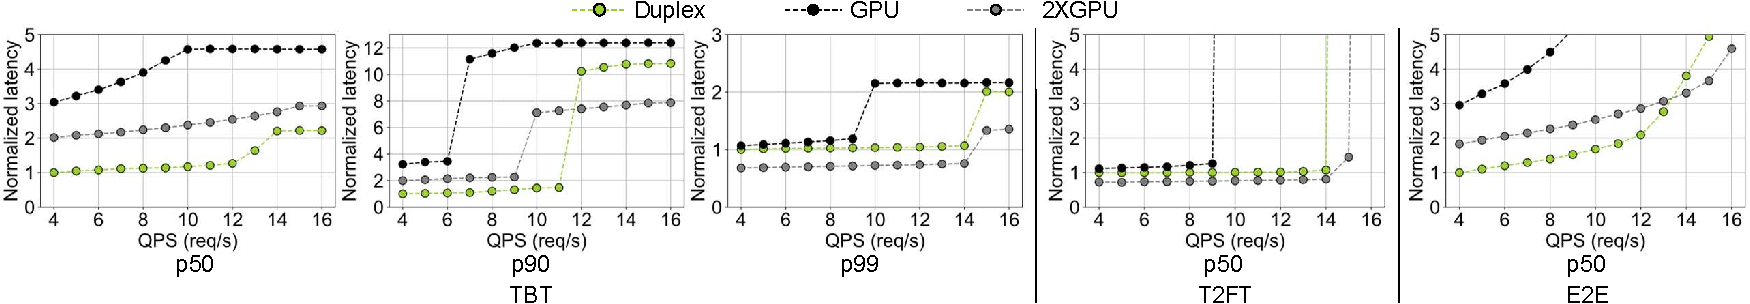
\includegraphics[width=1.00\textwidth]{figures/eval_qps_cam_ready.pdf}
  \vspace{-0.1in}
  \caption{
  The normalized latency (\tbt, \ttft, \ete) of \duplex, \gpu, and \doublegpu  for \mixtral varying queries per second (4 to 16). (\lin, \lout) is (4096, 512) and the maximum batch size is 128.
  }
  \label{fig:eval_qps}
  \vspace{-0.17in}
\end{figure*}


\subsection{Throughput Improvement of \duplex}
\label{sec:eval:duplex_throughput}
\duplex shows higher throughput than \gpu systems, with even \doublegpu in most cases by efficiently performing low~\opb MoE layers and attention layers using \lowp.
Fig.~\ref{fig:speedup_graph} shows the normalized throughput (tokens per second) of \duplex for various batch sizes and $(L_{in}, L_{out})$ configurations on three models compared to the \gpu.
To verify the performance enhancement of \duplex, we categorized \duplex into three configurations. 
\duplex is a device that uses only one of \highp or \lowp at any given time, as shown in Fig.~\ref{fig:duplex_operation_flow}(a) and (b). 
\duplexpe applies expert and attention co-processing, illustrated in Fig.~\ref{fig:duplex_operation_flow}(d). 
A device that incorporates tensor parallelism for MoE layers, as described in Section~\ref{sec:duplex_co-processing}, is referred to as \duplexpet.

\duplex already achieves up to 2.51$\times$ performance improvements compared to the baseline \gpu system, even showing the best performance for the $(L_{in}, L_{out}) =(4096, 4096)$ case of \mixtral.
There exist cases that \duplex outperforms the throughput of \doublegpu as \duplex utilizes greater memory bandwidth than that of \doublegpu in the low-\opb operations, which dominates the total execution time.

When only co-processing is applied, we observe an 1.04$\times$ on average in throughput compared to \duplex. 
Because each device processes fewer experts (two in the case of \mixtral and one for \grok), the benefits of expert co-processing are minimal.
While attention co-processing also reduces the latency of \mixedstage, it does not significantly improve throughput as \deconlystage dominates the stages in LLM inference.
\duplexpet enhances the effects of expert co-processing by employing tensor parallelism for experts as well, which increases the number of experts processed on each device, and increases throughput up to 1.36$\times$ and 2.67$\times$ compared to \duplex and \gpu.


\begin{figure}[!tb]
  \center
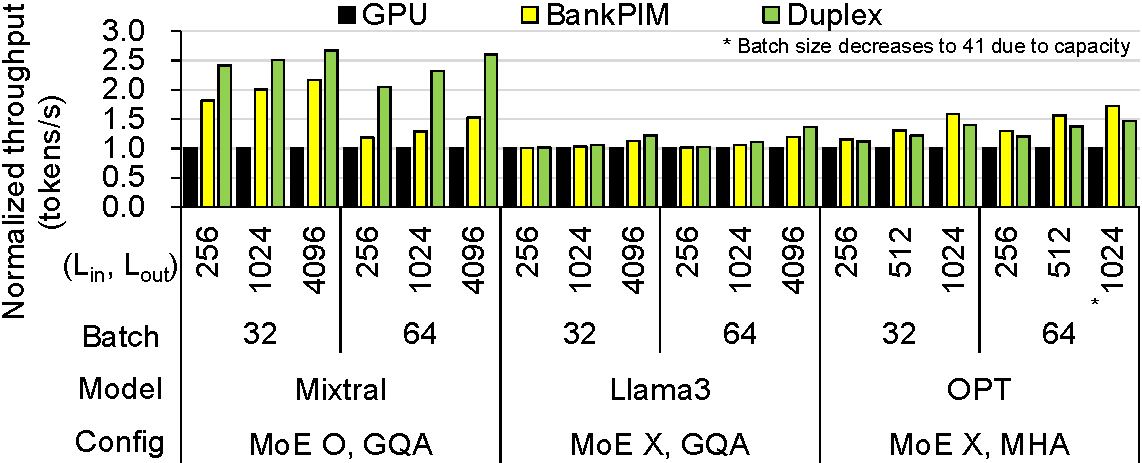
\includegraphics[width=1.0\columnwidth]{figures/eval_pim.pdf}
  \vspace{-0.15in}
  \caption{
  The normalized throughput of \duplex and \bankpim in \mixtral, \llama, and \opt for various (\lin, \lout) from (256, 256) to (4096, 4096) and batch sizes (32--64).
  }
  \label{fig:eval_ablation_study_pim}
  \vspace{-0.1in}
\end{figure}

In large systems, performance improvements may be limited due to communication overhead between devices and nodes.
\grok exhibits smaller performance improvements compared to the other models. 
This is due to \grok's larger model size, which necessitates using two nodes for LLM inference. 
Relatively low bandwidth between nodes increases communication overhead, consequently diminishing the acceleration benefits for the MoE layer and attention layer using \duplex.


\begin{figure*}[!tb]
  \center
  %0.98
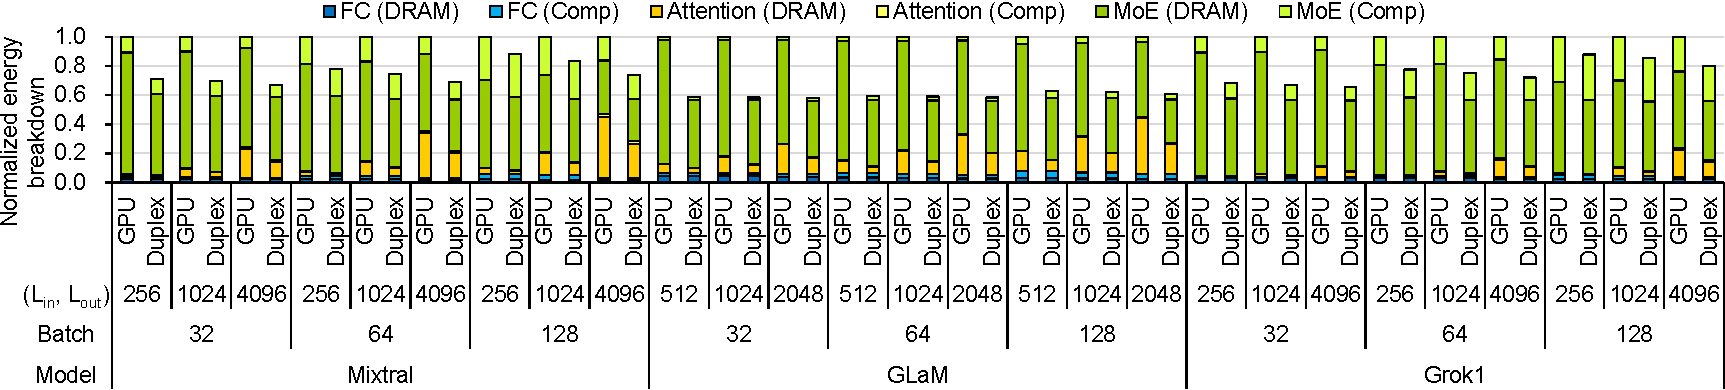
\includegraphics[width=1.0\textwidth]{figures/energy_breakdown_cam_ready.pdf}
  \vspace{-0.15in}
  \caption{
  The normalized energy breakdown of \mixtral, \glam, and \grok for various (\lin, \lout) from (256, 256) to (4096, 4096), and batch sizes (32--128).
  }
  \label{fig:energy_breakdown}
  \vspace{-0.12in}
\end{figure*}


\subsection{Latency Improvement of \duplex}
\label{sec:eval:duplex_latency}
\duplex significantly reduces the various types of latencies (\tbt, \ttft, \ete) over \gpu.
Fig.~\ref{fig:eval_latency_bar_graph} shows normalized latencies for \lin and \lout from 512 to 2048 in \glam with a batch size of 64.
On average, \duplex reduces the median \tbt value by 58.3\% by decreasing the execution times of the MoE layer and attention layer using \lowp compared to \gpu.
Further, \duplex achieves even lower median \tbt latency than \doublegpu.
The stage corresponding to the median \tbt latency is the \deconlystage, where the low~\opb MoE and attention layers dominate the execution time.
While \doublegpu utilizes twice as many processing units as \duplex to process the high-\opb FC layer quickly, \duplex can utilize twice the memory bandwidth as \doublegpu for low-\opb operations using \lowp.
By exploiting higher memory bandwidth using \lowp when processing dominant low~\opb operations in the \deconlystage, \duplex achieves a lower median \tbt latency than \doublegpu.

Even for median latencies of \ttft and 99th percentile for \tbt, which primarily occur in the \mixedstage well-suited to GPUs, \duplexpet achieves competitive latency improvements compared to \doublegpu.
When \lin is 512, \duplexpet could decrease the 99th percentile of \tbt and \ttft latencies up to 16.74\% and 26.17\% compared to \doublegpu. The \opb of the MoE layer in the \mixedstage is low enough to be accelerated by \lowp, making the expert and attention co-processing more effective.
When \lin is 2048, the \opb of the MoE layers in the mixed stage increases and the \lowp suffers from processing experts due to fewer processing units; thus, \duplexpet shows similar 99th percentile \tbt and \ttft with the \doublegpu.
By efficiently handling both \deconlystage and \mixedstage, \duplexpet reduces \ete latency by an average of 60.20\% and 35.38\% compared to \gpu and \doublegpu. 


To evaluate the performance of \duplex under different serving intensities, we measured the latency of \duplex, \gpu, and \doublegpu with varying QPS (see Fig.~\ref{fig:eval_qps}).
\duplex always exhibits better median \tbt latency than \doublegpu.
Because the median \tbt latency is generally achieved during the \deconlystage, \duplex outperforms \doublegpu by exploiting higher memory bandwidth using \lowp compared to \doublegpu.
At low QPS, \duplex outperforms \doublegpu in the 90th percentile of \tbt latency.
However, as QPS increases, \duplex shows higher latency compared to \doublegpu.
For high QPS, as the system processes more \mixedstage{s}, \doublegpu performs the \mixedstage better by utilizing twice as many computing units as \duplex, lowering tail \tbt latencies over \duplex.
If requests exceed the system's throughput, \ttft latency skyrockets due to the queuing delay.
\gpu cannot handle requests if more than 9 requests are injected per second.
\duplex, which processes the \deconlystage faster, can handle up to 14 requests per second, nearly equivalent to the capability of \doublegpu.
Thus, \duplex always outperforms \gpu and demonstrates similar or better performance across various QPS.


\subsection{Comparison with \bankpim Across Various LLMs}
\label{sec:eval:compare_pim}
\duplex outperforms \duplexbankpim by efficiently accelerating low-\opb (over 1) operations (see Fig.~\ref{fig:eval_ablation_study_pim}) in LLM with MoE and GQA.
\bankpim shows up to 2.17$\times$ higher throughput than \gpu in the batch size of 32 when (\lin,\lout) is 4096.
When the batch size decreases from 64 to 32, the \opb of the MoE layer is lowered, leading to relatively respectable performance improvements in \bankpim.
As the batch size increases, the processing units in \bankpim struggle with processing the MoE layers due to increased \opb.
\bankpim cannot efficiently process MoE layers when the batch size increases, leading to diminished performance gains and showing only 1.18$\times$ higher throughput compared to \gpu when (\lin,\lout) is 256 with a batch size of 64.
\duplex exploits \lowp equipped with more processing units than \bankpim, exhibiting 2.05$\times$ higher throughput than \gpu in the same configuration.
As the \deggrp of \mixtral is 4, \bankpim shows similar speedups compared to \duplex in processing the attention layer of decoding sequences, despite having higher amplified bandwidth.
By providing more adequate memory bandwidth and processing units than \bankpim, \duplex shows up to 1.80$\times$ higher throughput and 1.49$\times$ higher throughput on average compared to \bankpim in \mixtral.

\duplex still achieves acceptable speedups compared to \gpu in out-of-target models, such as conventional LLM models without MoE layers.
As the attention operations of decoding sequences are low~\opb operations, \duplex shows performance improvement. 
In \llama, which uses GQA (\deggrp = 8), \duplex performs better than \bankpim.
While \duplex can efficiently handle GQA, \bankpim suffers from a lack of computing units.
In the case of \opt, which utilizes MHA, \bankpim performs better than \duplex.
Because the \opb of MHA in the \deconlystage is extremely low, \bankpim processes the attention layer of the \deconlystage faster than \lowp by utilizing high internal memory bandwidth, leading to higher throughput than \duplex.
\begin{figure}[!tb]
  \center
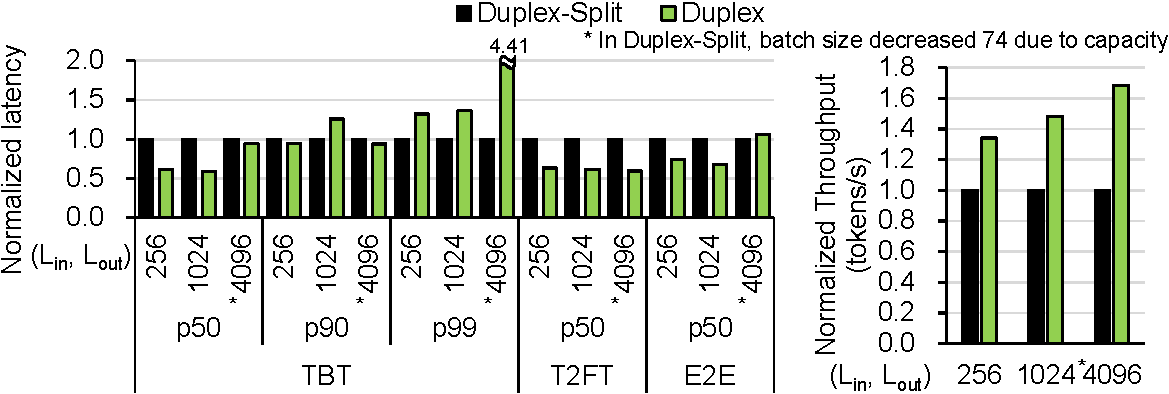
\includegraphics[width=1.0\columnwidth]{figures/eval_split.pdf}
  \caption{
  The normalized latency (\tbt, \ttft, \ete) of \mixtral for various (\lin, \lout) from (256, 256) to (4096, 4096) with a batch size of 128.
  \duplex and \duplexsplit each use a total of 4 \duplex devices. \duplexsplit processes each prefill stage and decoding stage with two \duplex units each.
  }
  \label{fig:split_duplex}
  \vspace{-0.15in}
\end{figure}



\subsection{Energy Consumption}
\label{sec:eval:energy}
\duplex reduces energy consumption by up to 33.28\%, 42.03\%, and 34.59\% for \mixtral, \glam, and \grok compared to \gpu.
Fig.~\ref{fig:energy_breakdown} shows normalized energy consumption for generating one token with \duplex and \gpu.
We can see that most of the energy is consumed in the MoE and attention layers.
\duplex reduces off-chip memory access energy in MoE and attention layer by leveraging \lowp.
The energy consumed by the attention layer rises as the sequence length increases, \duplex shows better energy efficiency in the long sequence lengths. 

In particular, energy efficiency deteriorates in \mixtral and \grok compared to \glam as the batch size increases. 
While \duplex reduces latency through co-processing, it consumes more energy by utilizing \highp, which uses more DRAM energy than \lowp. 
As \mixtral and \grok employ fewer experts than \glam, resulting in a higher \opb for the MoE layers in \mixtral and \grok than in \glam at the same batch size.
Thus, \duplex relies on \highp to process more experts in \mixtral and \grok compared to \glam, leading to relatively lower energy efficiency compared to \gpu when the batch size increases.

\subsection{Area Overhead}
\label{sec:eval:area_overhead}
The total overhead for processing units in \duplex for each \lowp stack is 17.80 mm$^2$, which accounts for 14.71\% of a 121 mm$^2$ HBM3 logic die~\cite{jssc-2022-hynix-hbm3}. 
The pitch of TSV was measured at 22 um~\cite{SKhynix-tsv-pitch}, and the number of TSVs per channel was conservatively scaled by increasing it to four times the number required per channel in conventional HBM3~\cite{SKhynix-tsv-pitch}. 
The added TSVs account for an area overhead of 10.89 mm$^2$. 
Each \lowp stack includes 32 GEMM modules, with each module comprising 512 FP16 MACs operating at 650MHz and a 8KB buffer, accounting for 3.02 mm$^2$.
Further, \lowp contains two 1MB buffers to store input vectors and temporal results, occupying 2.26 mm$^2$.
A softmax unit, which consists of a comparator tree, adders, exponential units, an adder tree, dividers, multipliers, and a total of 128 KB buffers, occupies 1.64 mm$^2$.
Considering that the area overhead ranges from 20\% to 27\%~\cite{isca-2021-hbm-pim, isscc-2022-aim}, \duplex demonstrates significant performance improvements with a lower area overhead.



